\section{Spørgsmål 1}

\subsection{Fokuspunkter}
\begin{itemize}
	\item Forklar principperne bag Entity/Relationship modellering.
	\begin{itemize}
		\item Herunder princippet for et Entity Relationsship Diagram (ERD)
	\end{itemize}
	\item Hvorledes opstilles et ER Diagram?
\end{itemize}

\subsection{Litteratur}
\begin{itemize}
	
	\item Fra teori: Database Modeling and Design. Logical Design 5'th Ed.
	\begin{itemize}
		\item Ch. 1 (p1 - 11)
		\item Ch. 2 (p13 - 34)
		\item Ch. 3 (p35 - 53)
		\item Ch. 4 (p55 - 84)
	\end{itemize}
	
	\item Fra Database eLearning: \url{http://db.grussell.org/index.html}.
	\begin{itemize}
		\item Database Analysis and ER Modelling.
		\begin{itemize}
			\item Database Analysis.
			\item Entity Relationship Modelling - 2.
			\item Advanced ER Mapping.
		\end{itemize}
	\end{itemize}
	
%	\item Fra wikipedia:
%	\begin{itemize}
%		\item 
%	\end{itemize}
%	
%	\item Fra Agile Data Home Page:
%	\begin{itemize}
%		\item 
%	\end{itemize}
\end{itemize}

\newpage

% must
\subsection{Forklar pincipperne bag Entity/Relationship modellering}

Generelt bruges \textit{Three-Level Database Model}. Denne anvendes når et design og fysisk implementering af databasen skal laves, ud fra nogle bestemte krav. 

\begin{enumerate}
	\item \textbf{Conceptual Data Model}\\
	Sparsom på detaljer. Giver overblik og ikke-teknisk-personale kan læse den.
	\item \textbf{Logical Data Model}\\
	Indeholder detaljer om Entities (tabeller) og Relationships (keys).
	\item \textbf{Physical Data Model}\\
	Er detaljeret nok til at databasen kan laves udfra denne. Indeholder information om tabeller, kolonner, keys, data-typer, validation rules, database triggers, stored procedures, domains, and access constraints.
\end{enumerate}

Ud fra dette skema den fysiske database genereres.

% must
\subsection{Forklar princippet for et Entity Relationsship Diagram (ERD)}

Et ER-diagram er en data modelleringsteknik som bruges til at gengive forholdet mellem entiteter i en databasen. Vil typisk bestå af følgende:

\begin{figure}[h]
	\centering
	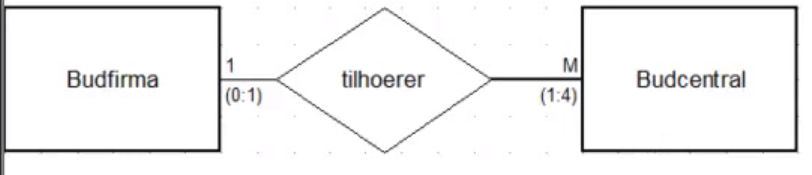
\includegraphics[width=0.8\linewidth]{figs/spm1/entity_in_relation}
	\caption{Eksempel på et ERD diagram.}
	\label{fig:erd}
\end{figure}

\subsubsection{Entity}
An entity exists physically or logically. An entity may be a physical object (house or car), an event (house sale or a car service), or a concept (transaction or order).

\subsubsection{Attributter}
Employee entity might have a Social Security Number (SSN) attribute.

\subsubsection{Relation}
A relationship captures how entities are related to one another. Relationships can be thought of as verbs, linking two or more nouns. Examples: a supervises relationship between an employee and a department, a performs relationship between an artist and a song.

\paragraph{Multiplicity}
Beskriver nedre- og øvre grænse for deltagelse i et relationship. Kan ses på figur~\ref{fig:erd}, som \textit{1} og \textit{M} over stregen.

\paragraph{Kardinalitet}
Angiver nøjagtigt hvor hvilket antal af en entitet, der er tilladt i en relation. Ses på figur~\ref{fig:erd} som \textit{1:N} og \textit{0:N} under stregen.

\begin{figure}[h]
	\centering
	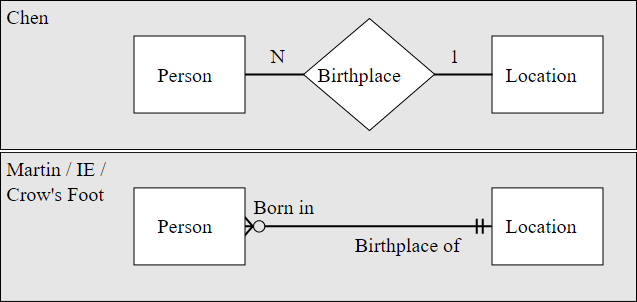
\includegraphics[width=0.8\linewidth]{figs/spm1/notation}
	\caption{Chen notation (øverst) og Crow's (nederst).}
	\label{fig:notation}
\end{figure}

\subsubsection{Keys}
For mere om nøgler se side~\pageref{sec:keys}.

\paragraph{Primærnøgle}
A primary key uniquely identifies each row/record in a database table. Primary keys \textbf{must} contain unique values. A primary key cannot be NULL.

A table can have only one primary key, which may consist of single or multiple fields. When multiple fields are used as a primary key, they are called a composite key.

\paragraph{Sekundærnøgle}
Foreign key is a field (or collection of fields) in one table that uniquely identifies a row of another table. 

In simpler words, the foreign key is defined in a second table, but it refers to the primary key in the first table.

% must
\subsection{Hvorledes opstilles et ER Diagram?}
Konstruktion af et ERD sker, som beskrevet af \href{http://db.grussell.org/section004.html#_Toc67114397}{pensum}, i følgende trin. Først læses specifikationen grundigt. Nødvendige antagelser dokumenteres. Derefter:

\begin{enumerate}
	\item Identify entities - list all potential entity types. These are the \textbf{object of interest} in the system. It is better to put too many entities in at this stage and them discard them later if necessary.
	
	\item Remove duplicate entities - Ensure that they really separate entity types.
	
	\begin{itemize}
		\item Do not include the system as an entity type. \item e.g. if modelling a library, the entity types might be books, borrowers, etc.
		\item The library is the system, thus should not be an entity type.
	\end{itemize}
	
	\item List the attributes of each entity (all properties to describe the entity which are relevant to the application).
	
	\begin{itemize}
		\item Ensure that the entity types are really needed.
		\item Are any of them just attributes of another entity type?
		\item If so keep them as attributes and cross them off the entity list.
		\item Do not have attributes of one entity as attributes of another entity!
	\end{itemize}
	
	\item Mark the primary keys.
	
	\begin{itemize}
		\item Which attributes uniquely identify instances of that entity type?
		\item This may not be possible for some weak entities.
	\end{itemize}
	
	\item Define the relationships.
	
	\begin{itemize}
		\item Examine each entity type to see its relationship to the others.
	\end{itemize}
	
	\item Describe the cardinality and optionality of the relationships.
	
	\begin{itemize}
		\item Examine the constraints between participating entities.
	\end{itemize}
	
	\item Remove redundant relationships.
	
	\begin{itemize}
		\item Examine the ER model for redundant relationships.
	\end{itemize}	
\end{enumerate}

\todo{find godt eksempel}
























